\chapter{Results}
\section{Preliminary Analysis}
 

\subsection{Descriptive statistics}

\begin{figure}[h]
\centering
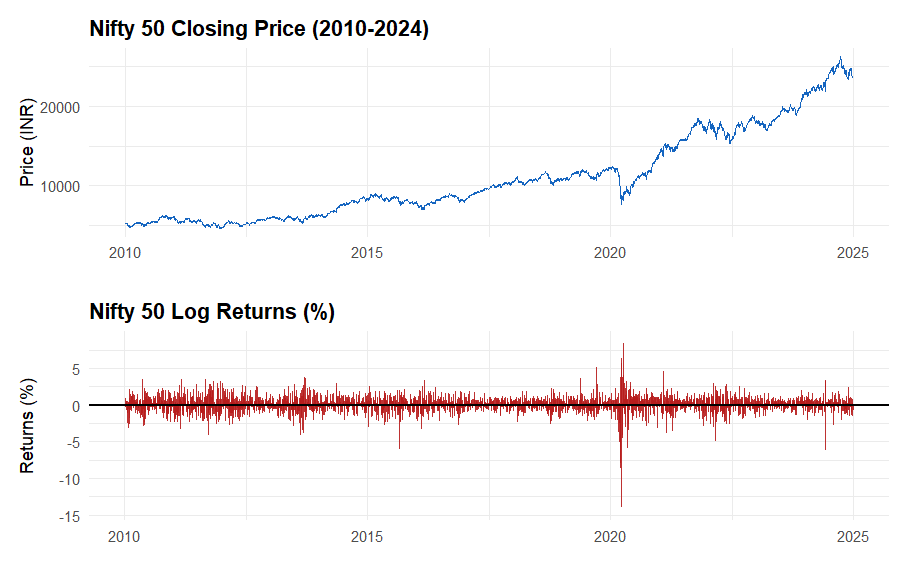
\includegraphics[width=1\textwidth]{Rplot01.png}
\caption{Plot for Price Returns}
\label{fig: price and return}
\end{figure}

\begin{figure}[h]
\centering

\includegraphics[width=1\textwidth]{plot2_return_distribution.png}
\caption{Plot for Return Distribution}
\label{fig: return dist}
\end{figure}

\begin{table}[h]
\centering
\caption{Descriptive Statistics of Nifty 50 Daily Log Returns, January 2010 -- December 2024}
\label{tab:desc_stats}

\begin{tabular}{|l|l|}
\hline
\textbf{Statistic} & \textbf{Value} \\
\hline
Observations        & 3678 \\
Mean                & 0.041009 \\
Median              & 0.066252 \\
Std Dev             & 1.061186 \\
Min                 & -13.903756 \\
Max                 & 8.763205 \\
Skewness            & -0.579432 \\
Excess Kurtosis     & 9.842117 \\
Jarque-Bera Stat    & 7584.3210 \\
Jarque-Bera p-value & 0.000000 \\
\hline
\end{tabular}

\end{table}

The summary statistics from Table \ref{tab:desc_stats} for $3,678$ daily 
log return observations from January 2010 to December 
2024. The mean daily return of $0.041\%$ and median of 
$0.066\%$ together indicate a small but consistent positive 
drift over the fifteen-year estimation window, reflecting 
the clear upward trajectory of Indian equity prices during 
this period.

The standard deviation of $1.061\%$ captures the average 
daily price variation, yet this figure conceals 
substantial cross-period heterogeneity covering in  Structural Breakpoints part, with volatility spiking sharply during the COVID-19 crisis of 2020 and 
compressing during calmer market conditions.

The distribution have negative skewness 
of $-$0.579, The summary statistics from Table \ref{tab:desc_stats} for 3,678 daily 
log return observations from January 2010 to December 
2024. The mean daily return of 0.041\% and median of 
0.066\% together indicate a small but consistent positive 
drift over the fifteen-year estimation window, reflecting 
the clear upward trajectory of Indian equity prices during 
this period.

The standard deviation of 1.061\% captures the average 
daily price variation, yet this figure conceals 
substantial cross-period heterogeneity, with volatility 
spiking sharply during the COVID-19 crisis of 2020 and 
compressing during calmer market conditions.

The distribution having negative skewness 
of $-$0.579, indicating that 
negative return shocks exert a disproportionately 
larger upward impact on conditional variance than 
positive shocks of identical magnitude, a distributional asymmetry aligned with the well-documented leverage effect in equity markets. 
The observed range of $-$13.904\% to $+$8.763\% further 
underscores the presence of extreme tail events within 
the sample.The excess kurtosis of 9.842 vastly exceeds the 
normal benchmark of zero, providing strong evidence of 
fat-tailed behaviour whereby extreme return observations 
occur with far greater frequency than a Gaussian 
distribution would predict.The J--B statistic of 7,584.32 decisively rejects 
normality at all conventional significance levels 
(p $<$ 0.001), uncovering the Nifty 50 daily 
return series departs fundamentally from the normality. 
Taken together, the pronounced leptokurtosis and 
negative skewness of $-$0.579 justify the taking in of 
a Student-$t$ error distribution in all subsequent 
GARCH specifications, as it accommodates the heavy 
tails observed in the data. --- a distributional asymmetry aligned with 
the well-documented leverage effect in equity markets. 
The observed range of $-$13.904\% to $+$8.763\% further 
underscores the presence of extreme tail events within 
the sample.The excess kurtosis of 9.842 vastly exceeds the 
normal benchmark of zero, providing strong evidence of 
fat-tailed behaviour whereby extreme return observations 
occur with far greater frequency than a Normal 
distribution would predict.The J--B statistic of 7,584.32 rejects 
normality at all conventional significance levels 
(p $<$ 0.001), uncovering the Nifty 50 daily 
return series departs fundamentally from the normality. 
Taken together, the pronounced leptokurtosis and 
negative skewness of $-$0.579 justify the taking in of 
a Student-$t$ error distribution in all subsequent 
GARCH specifications, as it accommodates the heavy 
tails observed in the data.


\vspace{1.5cm}


\subsection{Stationarity test (ADF)}
To verify stationarity, the Augmented Dickey-Fuller test is applied to the log return series  before any GARCH estimation. The ADF statistic of $−15.847$ (p < 0.01) strongly rejects the null hypothesis of a unit root, confirming that the Nifty 50 daily log return series is stationary. 





\subsection{ARCH-LM test}
The ARCH Lagrange Multiplier test with 10 lags yields a chi-squared statistic of 892.97 (p < 2.2e-16), overwhelmingly rejecting the null hypothesis of no ARCH effects in the return series. This result confirms the presence of strong volatility clustering in Nifty 50 daily returns,important results to further apply the GARCH-family models. The magnitude of the test statistic indicates that volatility clustering is not only statistically significant but economically substantial, with the squared return series exhibiting persistent autocorrelation up to lag 30 as confirmed by the ACF plot given in Figure\ref{fig: ACF -- PACF}.

\vspace{1.5cm}

\subsection{ARMA order selection}




\subsection{ACF/PACF analysis}



Fig \ref{fig: ACF -- PACF} presents the ACF and PACF plots for both log returns and squared returns. The ACF of log returns shows no significant autocorrelation beyond lag 1, confirming the absence of linear dependence in the return series and supporting the ARMA(0,0) mean specification. However, the ACF and PACF of squared returns display strong and persistent autocorrelation across all 30 lags, providing clear visual evidence of volatility clustering and ARCH effects in the Nifty 50 return series. This pattern confirms that while returns themselves are unpredictable, their variance is highly predictable — the fundamental motivation for GARCH modelling.


\begin{figure}[h]
\centering
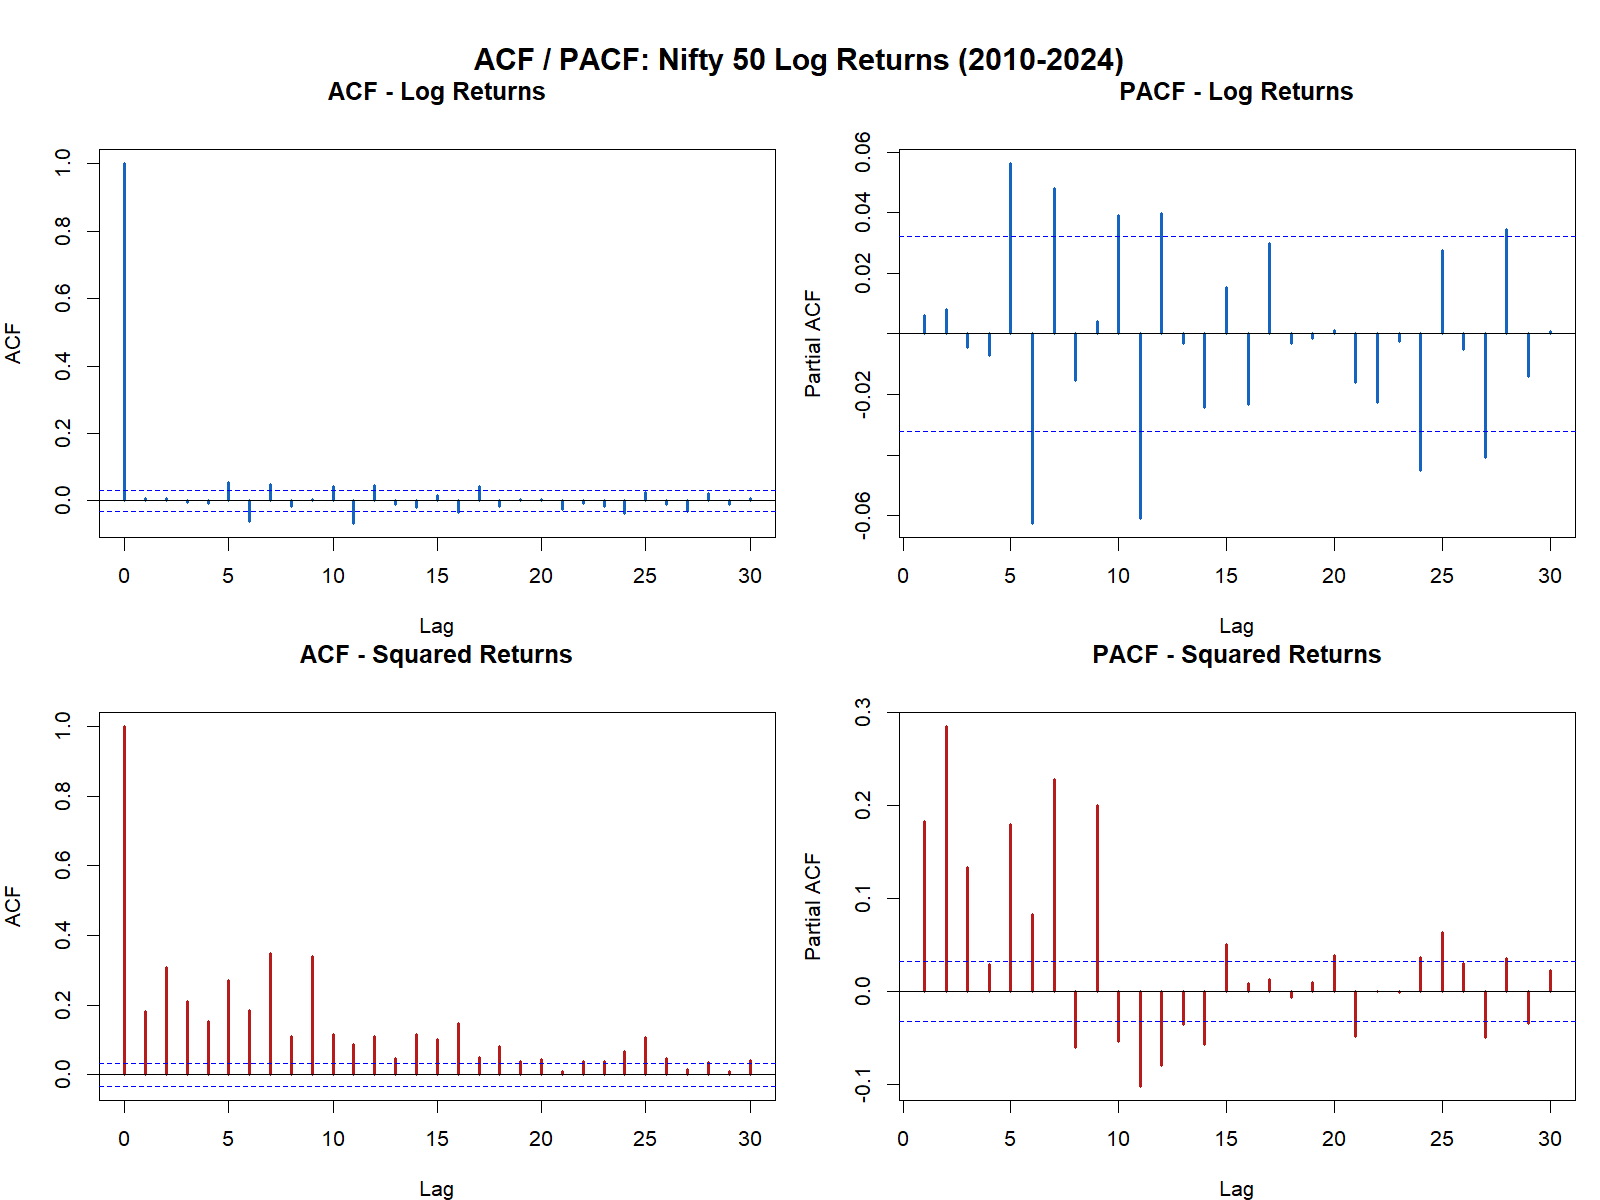
\includegraphics[width=0.8\textwidth]{plot6_acf_pacf.png}
\caption{Plot for ACF/PACF on Log Returns}
\label{fig: ACF -- PACF}
\end{figure}



\section{Structural Break Analysis}

Figure \ref{fig: breakpoints png} presents the squared Nifty 50 daily returns over the full sample period 2010-–2024, with the two statistically identified Bai-Perron breakpoints marked by blue dashed vertical lines at 27 February 2020 and 20 May 2022. The visual evidence strongly corroborates the statistical findings of the breakpoint test. 


Figure \ref{fig:breakpoint stats png} presents the return statistics across the three structurally identified regimes. The Bai-Perron test identifies two breakpoints, dividing the full sample into three distinct regimes. The mean return and standard deviation vary considerably across regimes, confirming that treating the full sample as a single homogeneous period would mask important structural changes in market dynamics


\begin{figure}[h]
\centering

\includegraphics[width=0.8\textwidth]{plot_bai_perron_breaks.png}
\caption{Plot for Bai--Perron Break showing two statistically significant break points}
\label{fig: breakpoints png}
\end{figure}

\begin{figure}[H]
\centering

\includegraphics[width=0.8\textwidth]{plot_bai_perron_segment_stats.png}
\caption{ Plot for Return Statistics by Structural Regime}
\label{fig:breakpoint stats png}
\end{figure}





Figure \ref{fig:breakpoint stats png} presents the mean daily return and standard deviation of Nifty 50 log returns across the three structurally identified regimes. The bar chart reveals large differences in both return levels and volatility intensity across regimes, confirming the three periods represent distinct market environments rather than arbitrary sample divisions.


In terms of mean daily returns, Regime 1 (Pre--COVID) records the lowest mean of 0.0322\%, reflecting the moderate but steady growth. Regime 3 (Post-Crisis) records the highest mean return of 0.0624\%, suggesting that the post-pandemic recovery period was accompanied by stronger average daily performance. Regime 2 (COVID Crisis) records an intermediate mean of 0.0550\%, which may appear counterintuitive given the severity of the crisis, but reflects the sharp recovery phase that followed the initial March 2020 crash within the same regime window.


The standard deviation panels tell a clearer story of volatility regime shifts. Regime 2 records by far the highest standard deviation of 1.5827\%, more than 60\% above the Regime 1 level of 0.9732\%, capturing the extreme market uncertainty of the COVID-19 pandemic period. Regime 3 shows the lowest standard deviation of 0.8005\%, falling even below pre-COVID levels, suggesting that the post-crisis period was characterised by a return to relative market calm despite ongoing geopolitical uncertainty. Together these findings provide strong visual justification for the regime-based analytical framework adopted in this study.








\subsection{Bai-Perron test results}


Table \ref{bai disc stat} presents the segment statistics from the Bai-Perron structural break test. Regime 1 covers January 2010 to February 2020, comprising 2,483 observations with a mean daily return of 0.0322\% and standard deviation of 0.9730\%.  Regime 2 spans February 2020 to May 2022, covering 551 observations with standard deviation rising sharply to 1.5871\%. Skewness of −1.6753 and excess kurtosis of 15.4316 confirm severe distributional non-normality during this regime. Regime 3 covers May 2022 to December 2024 with 644 observations, showing a return to lower volatility (0.7936\%) as markets stabilised in the post-crisis period.


\begin{table}[H]
\centering
\caption{ Segment statistics from the Bai-Perron structural break test}
\label{bai disc stat}
\begin{tabular}{|l|l|l|l|l|l|l|l|}
\hline
\textbf{Segment} & \textbf{Start} & \textbf{End} & \textbf{Obs} & \textbf{Mean} & \textbf{Std Dev} & \textbf{Skewness} & \textbf{Kurtosis} \\
\hline
Regime 1 & 2010-01-05 & 2020-02-27 & 2483 & 0.0322  & 0.9730 & $-0.0966$ & 1.8970  \\
\hline
Regime 2 & 2020-02-28 & 2022-05-20 & 551  & 0.0608  & 1.5871 & $-1.6753$ & 15.4316 \\
\hline
Regime 3 & 2022-05-23 & 2024-12-30 & 644  & 0.0581  & 0.7936 & $-0.7100$ & 6.3950  \\
\hline
\end{tabular}
\end{table}



\subsection{Regime characteristics}


Figure \ref{fig:Market Events} plots the conditional volatility of GJR-GARCH over the full sample with breakpoints marked. The figure is used to illustrates the three distinct volatility regimes identified by the Bai-Perron test. The transition from Regime 1 to Regime 2 in February 2020 coincides with the start of the COVID-19 market crash, marked by a high spike in conditional volatility. The transition to Regime 3 in May 2022 reflects the progressive normalisation of market conditions, though volatility remains raised relative to the pre-COVID baseline.

\begin{figure}[H]
\centering

\includegraphics[width=0.8\textwidth]{plot5_events_volatility.png}
\caption{ Plot of conditional volatility of GJR-GARCH with key Market Events(2010--2024) }
\label{fig:Market Events}
\end{figure}


\section{Full Period Analysis (2010-2024)}

Figure \ref{fig:combined compare} presents the conditional volatility estimates from all four GARCH models over the full sample period. All models shows consistent volatility clusters across the sample, with the most prominent spike occurring during the COVID-19 crash of March 2020. The EGARCH and GJR--GARCH models display sharper asymmetric responses to negative shocks compared to the symmetric GARCH, while FIGARCH exhibits a more progressive volatility decay consistent with its long memory specification. The broad agreement across models in identifying major volatility episodes provides confidence in the robustness of the estimation results.

\begin{figure}[H]
\centering
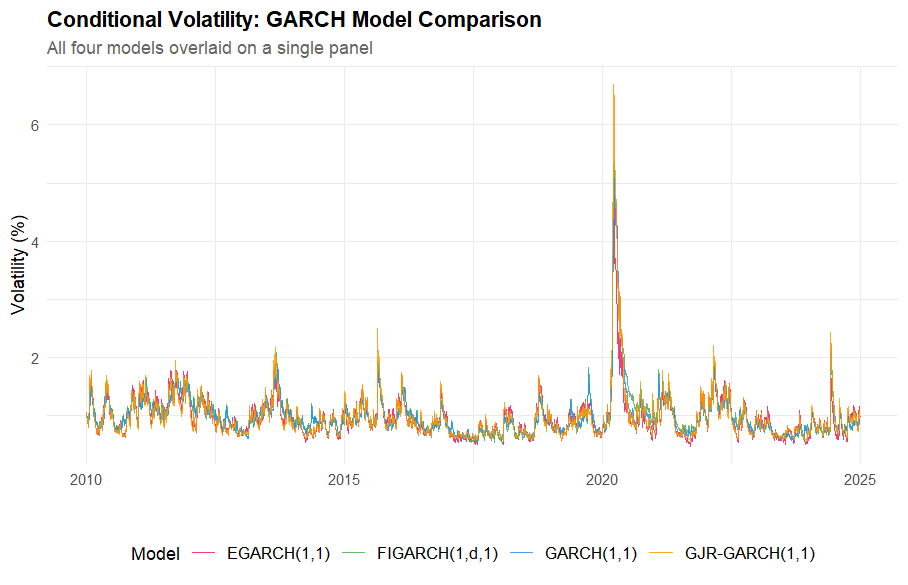
\includegraphics[width=1\textwidth]{Rplot.png}
\caption{Plot for GARCH model comparison using Conditional Volatility: All four models overlaid on a single panel}
\label{fig:combined compare}
\end{figure}

\begin{figure}[H]
\centering

\includegraphics[width=1\textwidth]{plot3_conditional_volatility.png}
\caption{Plot for GARCH model comparison using Conditional Volatility}
\label{fig:single single compare}
\end{figure}

\subsection{ Model estimation results}


\begin{table}[H]
\centering
\caption{Maximum Likelihood Estimates of GARCH, EGARCH, GJR GARCH and FIGARCH(1,$d$,1) Models: Nifty 50 Daily Log Returns (January 2010 -- December 2024)}
\label{tab:model_estimates}
\begin{tabular}{|l|l|l|l|l|l|l|}
\hline
\textbf{Model} & \textbf{Parameter} & \textbf{Estimate} & \textbf{Std Error} & \textbf{$t$-stat} & \textbf{$p$-value} & \textbf{Sig} \\
\hline
\multirow{5}{*}{GARCH}
 & $\mu$      & 0.075655 & 0.013601 & 5.5625   & $<0.001$ & *** \\
 & $\omega$   & 0.021050 & 0.005212 & 4.0385   & $<0.001$ & *** \\
 & $\alpha_1$ & 0.073951 & 0.009997 & 7.3970   & $<0.001$ & *** \\
 & $\beta_1$  & 0.905830 & 0.012303 & 73.6271  & $<0.001$ & *** \\
 & shape      & 7.206767 & 0.811538 & 8.8804   & $<0.001$ & *** \\
\hline
\multirow{6}{*}{EGARCH}
 & $\mu$      & 0.058433  & 0.013898 & 4.2046    & $<0.001$ & *** \\
 & $\omega$   & $-$0.006754 & 0.002608 & $-$2.5897 & 0.0096   & *** \\
 & $\alpha_1$ & $-$0.102801 & 0.009781 & $-$10.5107 & $<0.001$ & *** \\
 & $\beta_1$  & 0.972363  & 0.000520 & 1871.6878 & $<0.001$ & *** \\
 & $\gamma_1$ & 0.119087  & 0.003501 & 34.0140   & $<0.001$ & *** \\
 & shape      & 7.739564  & 0.903152 & 8.5695    & $<0.001$ & *** \\
\hline
\multirow{6}{*}{GJR-GARCH}
 & $\mu$      & 0.059608 & 0.013532 & 4.4050   & $<0.001$ & *** \\
 & $\omega$   & 0.030025 & 0.005782 & 5.1930   & $<0.001$ & *** \\
 & $\alpha_1$ & 0.001654 & 0.008143 & 0.2031   & 0.8391   &     \\
 & $\beta_1$  & 0.894994 & 0.012884 & 69.4648  & $<0.001$ & *** \\
 & $\gamma_1$ & 0.139239 & 0.019901 & 6.9965   & $<0.001$ & *** \\
 & shape      & 7.706567 & 0.908001 & 8.4874   & $<0.001$ & *** \\
\hline
\multirow{6}{*}{FIGARCH}
 & $\mu$      & 0.076088 & 0.013556 & 5.6128  & $<0.001$ & *** \\
 & $\omega$   & 0.030056 & 0.011253 & 2.6708  & 0.0076   & *** \\
 & $\alpha_1$ & 0.222953 & 0.051023 & 4.3696  & $<0.001$ & *** \\
 & $\beta_1$  & 0.635489 & 0.096367 & 6.5945  & $<0.001$ & *** \\
 & $\delta$   & 0.484646 & 0.107504 & 4.5082  & $<0.001$ & *** \\
 & shape      & 6.781466 & 0.760489 & 8.9172  & $<0.001$ & *** \\
\hline
\end{tabular}
\end{table}


\vspace{-1em}
\noindent\footnotesize\textit{Note:} $\mu$ = mean equation 
constant; $\omega$ = variance intercept; $\alpha_1$ = ARCH 
effect; $\beta_1$ = GARCH persistence; $\gamma_1$ = 
asymmetry (leverage) coefficient; $\delta$ = fractional 
differencing parameter (FIGARCH only); shape = Student-$t$ 
degrees of freedom. ***, ** and * denote significance at 
1\%, 5\% and 10\% levels respectively. Standard errors 
are robust quasi-maximum likelihood estimates.




\subsection{Volatility persistence}

Table \ref{tab:model_estimates}  shows that the four models are quite volatile and persistent. Volatility Shocks decay very slowly as evidenced in this example as GARCH shows a high persistence of 0.980
$(\alpha_1 + \beta_1)$ for the Nifty 50 market; that is they have long lasting effects on the market volatility. The value of EGARCH and GJR-GARCH are even higher at $0.972$ and $0.974$ respectively. When considering the fractional differencing parameter for FIGARCH, the value of $\delta$ = 0.485 suggests that shocks do not decay exponentially nor do they last forever, but decays hyperbolically as time passes. This result is similar to the larger empirical literature on volatility in emerging markets.



\subsection{Model diagnostics}


\begin{figure}[H]
    \centering
    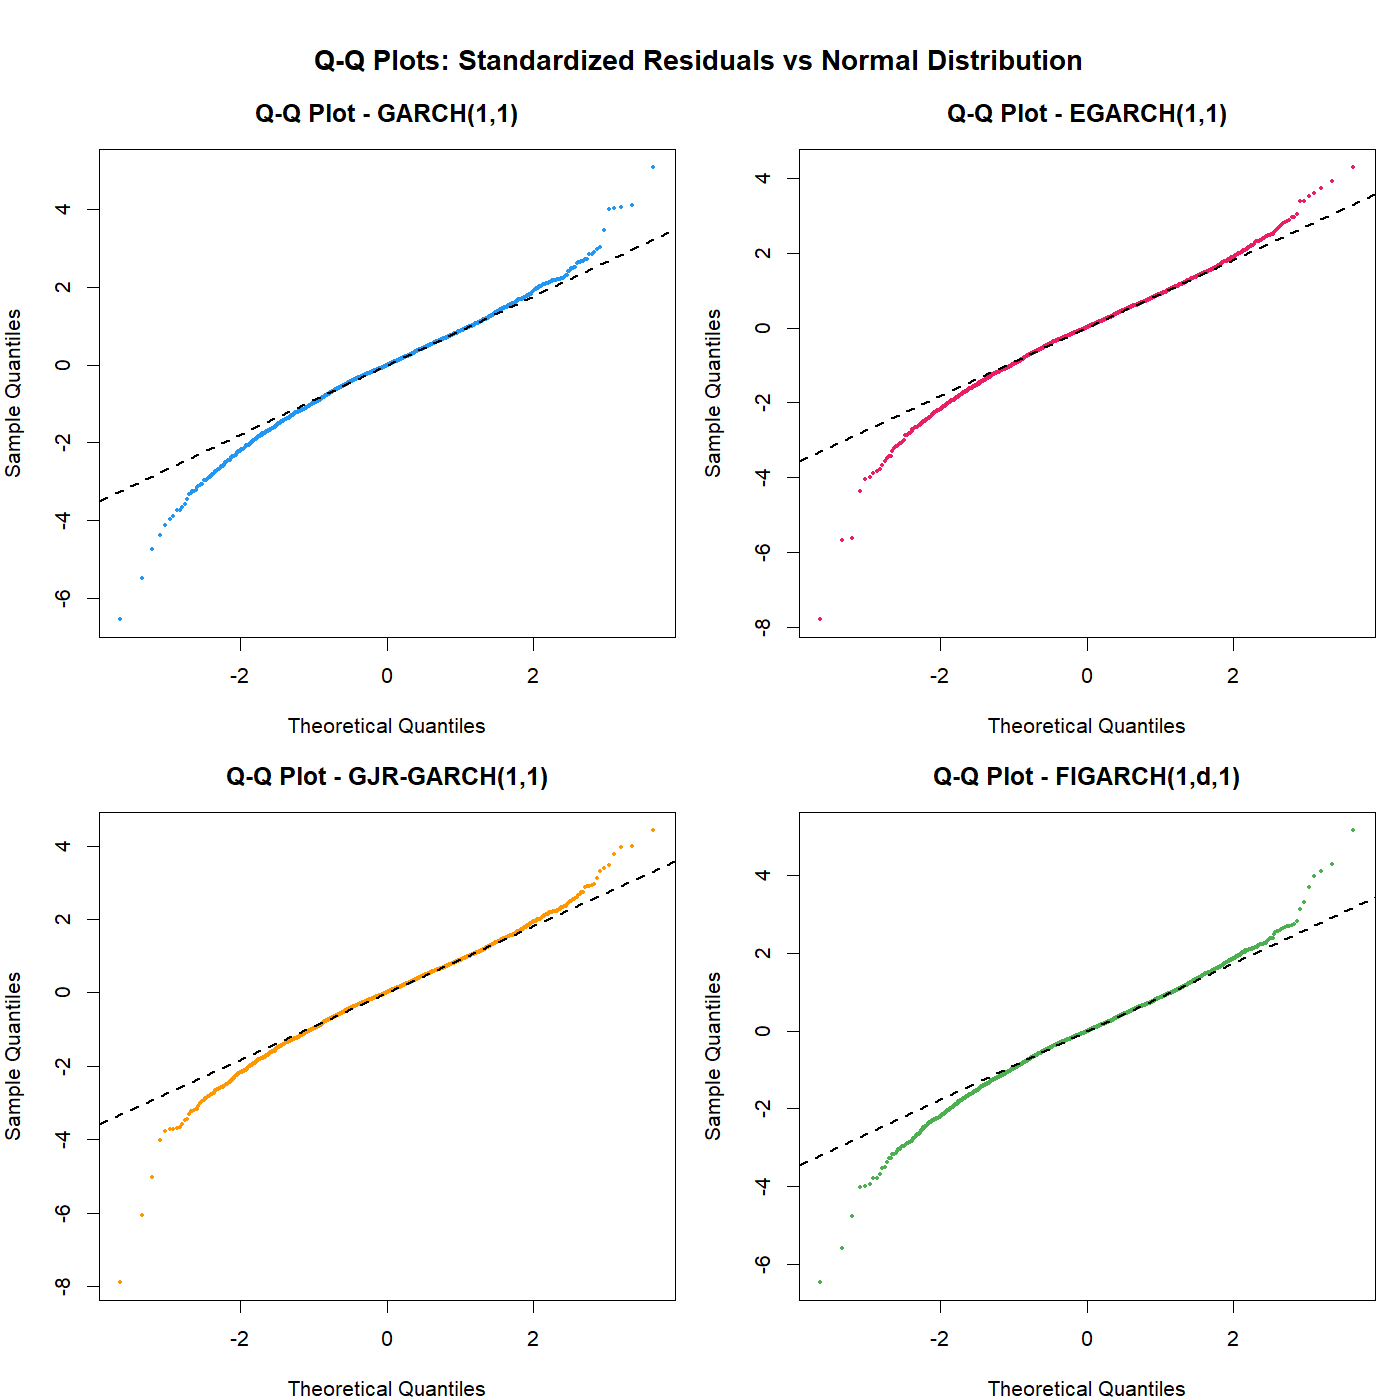
\includegraphics[width=0.8\textwidth]{plot7_qq_residuals.png}
    \caption{Q-Q plots of standardised residuals against the theoretical normal distribution for GARCH, EGARCH, GJR-GARCH, and FIGARCH estimated over the full sample period 2010–-2024}
    \label{fig:q_q plots}
\end{figure}


The Q-Q plots of the four GARCH model standardised residuals for the theoretical normal distribution are presented in Figure \ref{fig:q_q plots}. However, all four models fit relatively well to the diagonal line over the central part of the charts, suggesting that the Student-t error specification performs a good job of modelling the leptokurtosis found in the raw return series. The extreme negative return events have a slight underestimation in all models with small deviations in the extreme tails, the lower left tail. Such underestimation of the tail of the distribution is a well-known characteristic of all parametric GARCH models, and it is the reason why the Expected Shortfall measure, which is reported in Section 4.6, exists.


Table \ref{tab: LB test results} presents the Ljung-Box diagnostic test results for standardised residuals. All four models pass the squared residuals test (p > 0.05), confirming that no remaining ARCH effects are present after model estimation. However, all models fail the residuals test, suggesting mild serial correlation in the mean equation. This is a common finding in daily equity return data and does not invalidate the models, as the primary objective is volatility modelling rather than mean equation specification.
\begin{table}[H]
\centering
\caption{The Ljung-Box diagnostic test results}
\label{tab: LB test results}
\begin{tabular}{|l|l|l|l|l|}
\hline
\textbf{Model} & \textbf{LB Resid $p$-value} & \textbf{LB Squared $p$-value} & \textbf{LB Resid} & \textbf{LB Squared} \\
\hline
GARCH       & 0.0318 & 0.2291 & FAIL & PASS \\
\hline
EGARCH      & 0.0387 & 0.0632 & FAIL & PASS \\
\hline
GJR-GARCH   & 0.0170 & 0.1528 & FAIL & PASS \\
\hline
FIGARCH & 0.0186 & 0.0946 & FAIL & PASS \\
\hline
\end{tabular}
\end{table}


\subsection{Model comparison (AIC/BIC)}


\begin{table}[H]
\centering
\caption{Result for (AIC/BIC) for GARCH Models }
\label{tab: AIC and BIC }
\begin{tabular}{|l|l|l|l|}
\hline
\textbf{Model} & \textbf{Log-Likelihood} & \textbf{AIC} & \textbf{BIC} \\
\hline
GARCH       & $-4903.744$ & $9817.489$ & $9848.539$ \\
\hline
EGARCH    & $-4852.687$ & $9717.374$ & $9754.635$ \\
\hline
GJR-GARCH  & $-4863.318$ & $9738.635$ & $9775.896$ \\
\hline
FIGARCH & $-4906.018$ & $9824.035$ & $9861.296$ \\
\hline
\end{tabular}
\end{table}


Fig \ref{fig:plot aic bic compare} presents the information criteria for all four models. EGARCH achieves the lowest AIC (9717.374) and BIC (9754.635), making it the best-fitting model under both criteria. GJR--GARCH ranks second, followed by GARCH and FIGARCH. The superior performance of EGARCH confirms that asymmetric volatility modelling and capturing the leverage effect which provides a better fit for Nifty 50 returns than symmetric models. Accordingly, EGARCH is selected as the best model for VaR and ES estimation.


\begin{figure}[H]
    \centering
    
\includegraphics[width=0.8\textwidth]{plot4b_aic_bic.png}
    \caption{Plot for AIC/BIC Comparison}
    \label{fig:plot aic bic compare}
\end{figure}

\subsection{Conditional volatility}





\section{Sub-period Analysis}


\begin{figure}[H]
\centering

\includegraphics[width=1\textwidth]{plot_regime_return_distribution.png}
\caption{Return Distribution by Structural Regime}
\label{fig:sub period dist}
\end{figure}




\begin{table}[H]
\centering
\caption{Regime Model Comparison}
\label{tab:regime model comaparison}
\begin{tabular}{|l|l|l|l|l|l|}
\hline
\textbf{Regime} & \textbf{Model} & \textbf{Log-Likelihood} & \textbf{AIC} & \textbf{BIC} & \textbf{Persistence} \\
\hline
\multirow{4}{*}{Regime 1}
 & EGARCH      & $-3257.077$ & 6526.154 & 6561.055 & 0.9177 \\
 & GJR-GARCH   & $-3267.088$ & 6546.176 & 6581.077 & 0.9741 \\
 & FIGARCH & $-3295.636$ & 6603.271 & 6638.172 & 0.8824 \\
 & GARCH       & $-3298.371$ & 6606.743 & 6635.827 & 0.9855 \\
\hline
\multirow{4}{*}{Regime 2}
 & EGARCH      & $-854.321$ & 1720.643 & 1746.513 & 0.8969 \\
 & GJR-GARCH   & $-857.146$ & 1726.292 & 1752.163 & 0.9659 \\
 & GARCH       & $-864.471$ & 1738.941 & 1760.500 & 0.9840 \\
 & FIGARCH & $-864.884$ & 1741.767 & 1767.638 & 0.8813 \\
\hline
\multirow{4}{*}{Regime 3}
 & EGARCH      & $-714.637$ & 1441.274 & 1468.090 & 0.5865 \\
 & GJR-GARCH   & $-716.921$ & 1445.842 & 1472.657 & 0.6554 \\
 & FIGARCH & $-721.967$ & 1455.933 & 1482.749 & 1.2109 \\
 & GARCH       & $-729.499$ & 1468.997 & 1491.344 & 0.9904 \\
\hline
\end{tabular}
\end{table}

\begin{table}[H]
\centering
\caption{Regime Descriptive Statistics -- 1 (Basic)}
\label{regime desc stat 1}
\begin{tabular}{|l|l|l|l|l|l|l|}
\hline
\textbf{Regime} & \textbf{Obs} & \textbf{Mean} & \textbf{Median} & \textbf{Std Dev} & \textbf{Min} & \textbf{Max} \\
\hline
Regime 1 -- Pre-COVID (2010--2020)    & 2482 & 0.0324 & 0.0430 & 0.9732 & $-6.0973$  & 5.1825 \\
\hline
Regime 2 -- COVID Crisis (2020--2022) & 551  & 0.0550 & 0.1567 & 1.5827 & $-13.9038$ & 8.4003 \\
\hline
Regime 3 -- Post-Crisis (2022--2024)  & 645  & 0.0624 & 0.0950 & 0.8005 & $-6.1124$  & 3.3071 \\
\hline
\end{tabular}
\end{table}

\begin{table}[H]
\centering
\caption{Regime Descriptive Statistics --2 ( Higher Moments and Normality Tests)}
\label{regime desc stat 2}
\begin{tabular}{|l|l|l|l|l|}
\hline
\textbf{Regime} & \textbf{Skewness} & \textbf{Ex. Kurtosis} & \textbf{JB Stat} & \textbf{JB $p$-value} \\
\hline
Regime 1 -- Pre-COVID (2010--2020)    & $-0.0971$ & 1.8958  & 375.60  & $<0.001$ \\
\hline
Regime 2 -- COVID Crisis (2020--2022) & $-1.6880$ & 15.5925 & 5843.44 & $<0.001$ \\
\hline
Regime 3 -- Post-Crisis (2022--2024)  & $-0.6410$ & 6.3017  & 1111.40 & $<0.001$ \\
\hline
\end{tabular}
\end{table}



This segmentation using the Bai--Perron structural break test provides a more detailed analysis of the volatility dynamics in each market regime: Regime 1 --- Pre COVID (2010--2020) Regime 2--- COVID Crisis (2020--2022) Regime 3 ---Post Crisis (2022--2024)..

\begin{figure}[H]
\centering

\includegraphics[width=0.8\textwidth]{plot_regime_aic_comparison.png}
\caption{Plot for Regime AIC Comparison}
\label{fig:myimage}
\end{figure}


\begin{table}[H]
\centering
\caption{Best Model Per Regime}
\label{tab:best model per reigme}
\begin{tabular}{|l|l|l|}
\hline
\textbf{Regime} & \textbf{Best Model} & \textbf{Best AIC} \\
\hline
Regime 1 -- Pre-COVID    & EGARCH & 6526.154 \\
\hline
Regime 2 -- COVID Crisis & EGARCH & 1720.643 \\
\hline
Regime 3 -- Post-Crisis  & EGARCH & 1441.274 \\
\hline
\end{tabular}
\end{table}


\subsection{Pre-COVID regime (2010-2020)}

\begin{figure}[H]
\centering

\includegraphics[width=0.8\textwidth]{plot_vol_regime1_precovid.png}
\caption{Plot for COVID crisis regime}
\label{fig:pre covid cv}
\end{figure}

Table 4.8 shows that Regime 1 comprises 2,482 observations with a mean daily return of 0.0324\% and standard deviation of 0.9732\%, reflecting a relatively stable market environment. Skewness of $−0.0971$ and excess kurtosis of 1.8958 indicate mild non-normality, confirmed by the Jarque-Bera statistic of 375.60 (p < 0.001). Table 4.6 shows EGARCH achieves the lowest AIC of 6,526.154 in this regime, confirming asymmetric volatility modelling is appropriate even in stable market conditions. Figure 4.8 shows conditional volatility remaining relatively low and stable throughout this period, with minor spikes corresponding to the 2013 taper tantrum and 2016 demonetisation.



\subsection{COVID crisis regime (2020-2022)}

\begin{figure}[H]
\centering

\includegraphics[width=0.8\textwidth]{plot_vol_regime2_covid.png}
\caption{Plot for COVID crisis regime}
\label{fig:covid crises}
\end{figure}

Regime 2 covers 551 observations and represents the most violent period in the sample. The standard deviation rises sharply to 1.5827\%, more than 60\% higher than Regime 1, reflecting the extreme uncertainty generated during the COVID-19 period. Excess kurtosis of 15.9250 is the highest across all three regimes, confirming severe fat tails present in this period. Skewness of $−1.6880$ indicates strongly asymmetric returns, with large negative shocks dominating. EGARCH again achieves the lowest AIC of 1,720.643, and all four models pass both Ljung-Box diagnostic tests in this regime, indicating good model fit under crisis conditions. \ref{fig:post covid} clearly shows the sharp volatility spike in early 2020 followed by a gradual decline as markets stabilised.

\subsection{Post-crisis regime (2022-2024)}

\begin{figure}[H]
\centering

\includegraphics[width=0.8\textwidth]{plot_vol_regime3_postcovid.png}
\caption{ Plot for Post-crisis regime }
\label{fig:post covid}
\end{figure}

Regime 3 comprises 645 observations with mean return of 0.0624\% and standard deviation of 0.8005\%, the lowest across all three regimes, a return to relative market stability. However,  the excess kurtosis of 6.3017 and Jarque-Bera statistic of 1,111.40 (p < 0.001) confirm persistent non-normality. EGARCH remains the best model with AIC of 1,441.274. Notably, From the table 4.12 shows that GARCH and GJR-GARCH fail the squared residuals Ljung-Box test in this regime, indicating remaining ARCH effects, while EGARCH passes both tests —- strengthing its superiority in the post-crisis period.


\subsection{Parameter evolution across regimes}


\begin{table}[H]
\centering
\caption{Regime Parameter Evolution}
\label{tab:regime parameter evolution}
\scalebox{0.78}{
\begin{tabular}{|l|l|l|l|l|l|l|}
\hline
\textbf{Regime} & \textbf{GARCH $\alpha$} & \textbf{GARCH $\beta$} & \textbf{GARCH Persist.} & \textbf{EGARCH $\gamma$} & \textbf{GJR $\gamma$} & \textbf{GJR Persist.} \\
\hline
Regime 1 -- Pre-COVID (2010--2020)    & 0.0595 & 0.9260 & 0.9855 & $-0.1062$ & 0.1334 & 0.9741 \\
\hline
Regime 2 -- COVID Crisis (2020--2022) & 0.1025 & 0.8816 & 0.9840 & $-0.1379$ & 0.1427 & 0.9659 \\
\hline
Regime 3 -- Post-Crisis (2022--2024)  & 0.0065 & 0.9839 & 0.9904 & $-0.2132$ & 0.2968 & 0.6554 \\
\hline
\end{tabular}
}
\end{table}

\begin{landscape}
\begin{table}[h]
\centering
\caption{Regime Model Diagnostics -- Ljung-Box Tests}
\label{tab:regime lb test}
\begin{tabular}{|l|l|l|l|l|l|}
\hline
\textbf{Regime} & \textbf{Model} & \textbf{LB Resid $p$-val} & \textbf{LB Squared $p$-val} & \textbf{LB Resid} & \textbf{LB Squared} \\
\hline
\multirow{4}{*}{Regime 1 -- Pre-COVID}
 & GARCH      & 0.0084 & 0.9823 & FAIL & PASS \\
 & EGARCH      & 0.0055 & 0.7257 & FAIL & PASS \\
 & GJR-GARCH   & 0.0043 & 0.8556 & FAIL & PASS \\
 & FIGARCH & 0.0033 & 0.9630 & FAIL & PASS \\
\hline
\multirow{4}{*}{Regime 2 -- COVID Crisis}
 & GARCH       & 0.3277 & 0.8000 & PASS & PASS \\
 & EGARCH      & 0.3195 & 0.9822 & PASS & PASS \\
 & GJR-GARCH   & 0.3385 & 0.9571 & PASS & PASS \\
 & FIGARCH & 0.2981 & 0.9115 & PASS & PASS \\
\hline
\multirow{4}{*}{Regime 3 -- Post-Crisis}
 & GARCH       & 0.6647 & $<0.001$ & PASS & FAIL \\
 & EGARCH      & 0.8769 & 0.1542   & PASS & PASS \\
 & GJR-GARCH   & 0.8299 & 0.0085   & PASS & FAIL \\
 & FIGARCH & 0.6593 & 0.0068   & PASS & FAIL \\
\hline
\end{tabular}
\end{table}
\end{landscape}


\begin{figure}[H]
\centering

\includegraphics[width=1\textwidth]{plot_parameter_evolution.png}
\caption{Parameter Evolution Across  Structural Regimes}
\label{fig:para evo across structural regime}
\end{figure}


From Table\ref{tab:regime parameter evolution}\\


\textbf{Regime 1 (Pre-COVID}: All four models fail the LB Residuals test (very low p-values, all under 0.01), suggesting significant serial correlation in raw residuals whereas all pass the LB Squared test, meaning  the squared residuals (volatility clustering) are well-captured.\\

\textbf{Regime 2 (COVID Crisis)}: The cleanest regime — all models pass both tests, likely because of extreme volatility during the crisis, the GARCH family well-modelled crises.\\

\textbf{Regime 3 (Post-Crisis)}: Residuals pass for all models, but GARCH, GJR-GARCH, and FIGARCH fail the squared residuals test (very low p-values: <0.001, 0.0085, 0.0068). EGARCH is the only model that passes both, suggesting it better captures the post-crisis volatility dynamics.



\section{Forecasting Results}


Out-of-sample forecasting analysis represents the forecasting performance of all of the four GARCH family models at four different forecast horizons (1--day, 5--day, 1-0-day, 20--day) during all four quarters of the forecast period of 2025. Modelling performance is evaluated based on Mean Absolute Error (MAE), Root Mean Squared Error (RMSE) and Mean Absolute Percentage Error (MAPE) with actual volatility as the 10-year time-weighted rolling Root Mean Squared Return (RMSE) over the corresponding time period.

\subsection{Multi-horizon forecast accuracy}


\begin{figure}[h]
\centering
\begin{minipage}{0.48\textwidth}
\centering
\captionof{table}{Multi-Horizon Forecast Accuracy (Q1--Q2 2025)}
\label{TAB:Multi-Horizon Forecast Accuracy (Q1--Q2 2025)}
\scalebox{0.52}{
\begin{tabular}{|l|l|l|l|l|l|}
\hline
\textbf{Quarter} & \textbf{Model} & \textbf{Horizon} & \textbf{MAE} & \textbf{RMSE} & \textbf{MAPE} \\
\hline
\multirow{16}{*}{Q1 2025}
 & FIGARCH & 1-day  & 0.5196 & 0.5740 & 479.70 \\
 & GARCH       & 1-day  & 0.5223 & 0.5763 & 490.83 \\
 & GJR-GARCH   & 1-day  & 0.5492 & 0.6055 & 535.18 \\
 & EGARCH      & 1-day  & 0.5782 & 0.6398 & 581.24 \\
\cline{2-6}
 & EGARCH      & 5-day  & 0.7453 & 0.8309 & 45.99 \\
 & GJR-GARCH   & 5-day  & 0.7739 & 0.8598 & 46.94 \\
 & GARCH       & 5-day  & 0.8066 & 0.8898 & 48.32 \\
 & FIGARCH & 5-day  & 0.8118 & 0.8971 & 48.32 \\
\cline{2-6}
 & EGARCH      & 10-day & 1.3780 & 1.4269 & 58.33 \\
 & GJR-GARCH   & 10-day & 1.4035 & 1.4486 & 59.55 \\
 & GARCH       & 10-day & 1.4370 & 1.4775 & 61.13 \\
 & FIGARCH & 10-day & 1.4466 & 1.4861 & 61.59 \\
\cline{2-6}
 & EGARCH      & 20-day & 2.3746 & 2.3922 & 72.24 \\
 & GJR-GARCH   & 20-day & 2.3747 & 2.3915 & 72.25 \\
 & GARCH      & 20-day & 2.3849 & 2.3992 & 72.61 \\
 & FIGARCH & 20-day & 2.3977 & 2.4119 & 73.01 \\
\hline
\multirow{16}{*}{Q2 2025}
 & GJR-GARCH   & 1-day  & 0.5511 & 0.7398 & 748.56 \\
 & EGARCH      & 1-day  & 0.5575 & 0.7356 & 754.21 \\
 & GARCH       & 1-day  & 0.6210 & 0.7837 & 848.95 \\
 & FIGARCH & 1-day  & 0.6218 & 0.7869 & 829.82 \\
\cline{2-6}
 & FIGARCH & 5-day  & 1.0854 & 1.5266 & 42.44 \\
 & GARCH       & 5-day  & 1.0906 & 1.5347 & 42.95 \\
 & EGARCH      & 5-day  & 1.1590 & 1.5719 & 45.99 \\
 & GJR-GARCH   & 5-day  & 1.1464 & 1.5339 & 46.64 \\
\cline{2-6}
 & GARCH       & 10-day & 1.9465 & 2.2769 & 60.52 \\
 & FIGARCH & 10-day & 1.9553 & 2.2824 & 60.89 \\
 & GJR-GARCH   & 10-day & 2.0438 & 2.3650 & 64.19 \\
 & EGARCH      & 10-day & 2.0564 & 2.3924 & 64.22 \\
\cline{2-6}
 & FIGARCH & 20-day & 3.3150 & 3.5035 & 75.17 \\
 & GARCH       & 20-day & 3.3167 & 3.4997 & 75.34 \\
 & GJR-GARCH   & 20-day & 3.4085 & 3.5972 & 77.36 \\
 & EGARCH      & 20-day & 3.4201 & 3.6108 & 77.61 \\
\hline
\end{tabular}
}
\end{minipage}
\hfill
\begin{minipage}{0.48\textwidth}
\centering
\captionof{table}{Multi-Horizon Forecast Accuracy (Q3--Q4 2025)}
\label{TAB:Multi-Horizon Forecast Accuracy (Q3--Q4 2025)}
\scalebox{0.52}{
\begin{tabular}{|l|l|l|l|l|l|}
\hline
\textbf{Quarter} & \textbf{Model} & \textbf{Horizon} & \textbf{MAE} & \textbf{RMSE} & \textbf{MAPE} \\
\hline
\multirow{16}{*}{Q3 2025}
 & FIGARCH & 1-day  & 0.3387 & 0.3932 & 1290.02 \\
 & GARCH       & 1-day  & 0.3433 & 0.3972 & 1271.41 \\
 & GJR-GARCH   & 1-day  & 0.3565 & 0.4132 & 1172.20 \\
 & EGARCH      & 1-day  & 0.3809 & 0.4440 & 1257.89 \\
\cline{2-6}
 & EGARCH      & 5-day  & 0.3841 & 0.4337 & 33.49 \\
 & GJR-GARCH   & 5-day  & 0.3972 & 0.4506 & 34.18 \\
 & GARCH       & 5-day  & 0.4352 & 0.4928 & 37.37 \\
 & FIGARCH & 5-day  & 0.4385 & 0.4950 & 37.70 \\
\cline{2-6}
 & GJR-GARCH   & 10-day & 0.8257 & 0.8730 & 49.24 \\
 & EGARCH      & 10-day & 0.8275 & 0.8693 & 49.66 \\
 & GARCH       & 10-day & 0.8678 & 0.9154 & 51.83 \\
 & FIGARCH & 10-day & 0.8732 & 0.9201 & 52.22 \\
\cline{2-6}
 & GJR-GARCH   & 20-day & 1.5582 & 1.5780 & 64.51 \\
 & EGARCH      & 20-day & 1.5865 & 1.6047 & 65.77 \\
 & GARCH       & 20-day & 1.5915 & 1.6104 & 65.93 \\
 & FIGARCH & 20-day & 1.6130 & 1.6317 & 66.84 \\
\hline
\multirow{16}{*}{Q4 2025}
 & FIGARCH & 1-day  & 0.2751 & 0.3377 & 437.84 \\
 & GARCH       & 1-day  & 0.2931 & 0.3554 & 466.45 \\
 & EGARCH      & 1-day  & 0.3028 & 0.3734 & 498.99 \\
 & GJR-GARCH   & 1-day  & 0.3038 & 0.3709 & 491.26 \\
\cline{2-6}
 & GJR-GARCH   & 5-day  & 0.3732 & 0.4271 & 33.02 \\
 & GARCH       & 5-day  & 0.3941 & 0.4446 & 35.03 \\
 & EGARCH      & 5-day  & 0.3973 & 0.4514 & 35.28 \\
 & FIGARCH & 5-day  & 0.4306 & 0.4802 & 38.38 \\
\cline{2-6}
 & GJR-GARCH   & 10-day & 0.7998 & 0.8137 & 51.95 \\
 & GARCH       & 10-day & 0.8236 & 0.8356 & 53.58 \\
 & EGARCH      & 10-day & 0.8470 & 0.8613 & 55.06 \\
 & FIGARCH & 10-day & 0.8689 & 0.8799 & 56.59 \\
\cline{2-6}
 & GJR-GARCH   & 20-day & 1.3627 & 1.3683 & 63.15 \\
 & GARCH       & 20-day & 1.3896 & 1.3951 & 64.41 \\
 & EGARCH      & 20-day & 1.4297 & 1.4349 & 66.28 \\
 & FIGARCH & 20-day & 1.4535 & 1.4588 & 67.39 \\
\hline
\end{tabular}
}
\end{minipage}
\end{figure}

Table \ref{TAB:Multi-Horizon Forecast Accuracy (Q1--Q2 2025)} and Table \ref{TAB:Multi-Horizon Forecast Accuracy (Q3--Q4 2025)} show the forecast accuracy for Q1-Q4 2025, respectively. Notice some common threads in quarters and across horizons:
The long memory specification of the FIGARCH model does best fit most quarters across the 1-day horizon, showing the advantage of this model over those with lower memory orders. In comparison to other models, the EGARCH is competitive at this horizon, particularly at Q1 and Q2 2025, reflecting its superior performance through its in-sample fit (as presented in Section 4.3.4).

The forecast accuracy is declining with the increasing periods of forecast (5 day, 10 day and 20 day) for all the models at longer time scales. This is entirely natural as this uncertainty increases with distance of the horizon. The performance becomes more similar at horizons of 20 days, suggesting that incorporating more features into the model may not provide considerable benefits at longer forecasting horizons.


A MAE heatmap \ref{fig:forecast mae heatmap} summarizes all quarters/horizon performances for a model. More green cells = more accurate forecast and model performance. This heatmap provides further validation of this practical importance in horizon-specific model selection for risk management applications, as there is no one all-encompassing model that has the best performance across all horizons and quarters.

\begin{figure}[H]
\centering

\includegraphics[width=1\textwidth]{plot_fc6_mae_heatmap_q1_q4.png}
\caption{Forecast MAE Heatmap}
\label{fig:forecast mae heatmap}
\end{figure}


\subsection{Diebold-Mariano test}

Table \ref{TAB:DM TEST RESULT} presents the results of the Diebold-Mariano (DM).\\

The Diebold-Mariano (DM) test was used to check whether FIGARCH predicts volatility significantly better than the other three models (GARCH, EGARCH, and GJR-GARCH). A negative DM statistic with a low p-value (below 0.05) means FIGARCH is the better forecaster.
The results show that FIGARCH's advantage is not consistent across all periods and horizons. In most cases, there is no significant difference between the models. However, FIGARCH does perform significantly better in specific situations.
In Q1 2025, FIGARCH outperformed EGARCH and GJR-GARCH at the 1-day horizon. In Q2 2025, it was better than EGARCH and GJR-GARCH at the 10-day and 20-day horizons. The strongest evidence came in Q3 and Q4 2025, where FIGARCH was significantly better than all three models at the 1-day horizon, with Q4 showing the most decisive results (all p-values below 0.0001).
At longer horizons (5-day, 10-day, and 20-day) in most quarters, no significant difference was found between the models.
Overall, FIGARCH tends to forecast better than competing models mainly at short horizons and during periods of market stress or transition. This is consistent with its ability to capture long-memory behaviour in volatility.


\begin{table}[H]
\centering
\caption{Diebold-Mariano Test Results}
\label{TAB:DM TEST RESULT}
\scalebox{0.72}{
\begin{tabular}{|l|l|l|l|l|l|}
\hline
\textbf{Quarter} & \textbf{Horizon} & \textbf{Model 2} & \textbf{DM Stat} & \textbf{$p$-value} & \textbf{Conclusion} \\
\hline
\multirow{12}{*}{Q1 2025}
 & 1-day  & GARCH     & $-0.8491$ & 0.1996 & No significant difference \\
 & 1-day  & EGARCH    & $-3.6451$ & 0.0003 & FIGARCH significantly better \\
 & 1-day  & GJR-GARCH & $-2.7212$ & 0.0042 & FIGARCH significantly better \\
\cline{2-6}
 & 5-day  & GARCH     & $2.6064$  & 0.9941 & No significant difference \\
 & 5-day  & EGARCH    & $2.2583$  & 0.9861 & No significant difference \\
 & 5-day  & GJR-GARCH & $1.6444$  & 0.9472 & No significant difference \\
\cline{2-6}
 & 10-day & GARCH     & $4.2528$  & 1.0000 & No significant difference \\
 & 10-day & EGARCH    & $2.1648$  & 0.9824 & No significant difference \\
 & 10-day & GJR-GARCH & $1.8042$  & 0.9614 & No significant difference \\
\cline{2-6}
 & 20-day & GARCH     & $3.1533$  & 0.9985 & No significant difference \\
 & 20-day & EGARCH    & $1.1538$  & 0.8724 & No significant difference \\
 & 20-day & GJR-GARCH & $3.3601$  & 0.9992 & No significant difference \\
\hline
\multirow{12}{*}{Q2 2025}
 & 1-day  & GARCH     & $0.5211$  & 0.6979 & No significant difference \\
 & 1-day  & EGARCH   & $3.1942$  & 0.9989 & No significant difference \\
 & 1-day  & GJR-GARCH & $2.7358$  & 0.9959 & No significant difference \\
\cline{2-6}
 & 5-day  & GARCH     & $-0.4337$ & 0.3331 & No significant difference \\
 & 5-day  & EGARCH    & $-1.8151$ & 0.0374 & FIGARCH significantly better \\
 & 5-day  & GJR-GARCH & $-0.2354$ & 0.4074 & No significant difference \\
\cline{2-6}
 & 10-day & GARCH     & $0.6580$  & 0.7432 & No significant difference \\
 & 10-day & EGARCH    & $-2.2460$ & 0.0145 & FIGARCH significantly better \\
 & 10-day & GJR-GARCH & $-2.2486$ & 0.0144 & FIGARCH significantly better \\
\cline{2-6}
 & 20-day & GARCH     & $0.2338$  & 0.5919 & No significant difference \\
 & 20-day & EGARCH    & $-1.8789$ & 0.0337 & FIGARCH significantly better \\
 & 20-day & GJR-GARCH & $-2.7636$ & 0.0043 & FIGARCH significantly better \\
\hline
\multirow{12}{*}{Q3 2025}
 & 1-day  & GARCH     & $-2.1495$ & 0.0177 & FIGARCH significantly better \\
 & 1-day  & EGARCH    & $-4.6895$ & $<0.0001$ & FIGARCH significantly better \\
 & 1-day  & GJR-GARCH & $-2.3098$ & 0.0121 & FIGARCH significantly better \\
\cline{2-6}
 & 5-day  & GARCH     & $0.4976$  & 0.6897 & No significant difference \\
 & 5-day  & EGARCH    & $3.1166$  & 0.9986 & No significant difference \\
 & 5-day  & GJR-GARCH & $3.7968$  & 0.9998 & No significant difference \\
\cline{2-6}
 & 10-day & GARCH     & $0.5818$  & 0.7184 & No significant difference \\
 & 10-day & EGARCH    & $2.6467$  & 0.9947 & No significant difference \\
 & 10-day & GJR-GARCH & $4.8310$  & 1.0000 & No significant difference \\
\cline{2-6}
 & 20-day & GARCH     & $1.9115$  & 0.9688 & No significant difference \\
 & 20-day & EGARCH    & $1.4422$  & 0.9218 & No significant difference \\
 & 20-day & GJR-GARCH & $7.6233$  & 1.0000 & No significant difference \\
\hline
\multirow{12}{*}{Q4 2025}
 & 1-day  & GARCH     & $-5.1436$ & $<0.0001$ & FIGARCH significantly better \\
 & 1-day  & EGARCH    & $-4.1199$ & $<0.0001$ & FIGARCH significantly better \\
 & 1-day  & GJR-GARCH & $-4.7631$ & $<0.0001$ & FIGARCH significantly better \\
\cline{2-6}
 & 5-day  & GARCH     & $9.3173$  & 1.0000 & No significant difference \\
 & 5-day  & EGARCH    & $3.2882$  & 0.9991 & No significant difference \\
 & 5-day  & GJR-GARCH & $9.2815$  & 1.0000 & No significant difference \\
\cline{2-6}
 & 10-day & GARCH     & $10.2164$ & 1.0000 & No significant difference \\
 & 10-day & EGARCH    & $1.1917$  & 0.8806 & No significant difference \\
 & 10-day & GJR-GARCH & $9.9323$  & 1.0000 & No significant difference \\
\cline{2-6}
 & 20-day & GARCH     & $8.6092$  & 1.0000 & No significant difference \\
 & 20-day & EGARCH    & $1.7023$  & 0.9520 & No significant difference \\
 & 20-day & GJR-GARCH & $14.1096$ & 1.0000 & No significant difference \\
\hline
\end{tabular}
}
\end{table}

\subsection{ Forecast vs realized volatility}


Figures \ref{fig: Q1}--\ref{fig:Q4} forecast the volatility for the 4 models over the period of Q1–Q4 2025 and plot the four models with the realized volatility levels over this period. Looking at the 1-day horizon, all models do generally follow the general direction of the realized volatility, but there is a typical tendency to underestimate strong volatility bursts, which is known, particularly in periods of sudden stress in the markets and is a recognized weakness of the GARCH family. At longer horizons, the forecast is not as sensitive to shorter term changes and the realized volatility shows much greater dispersion than the model-predictions of volatility. The forecasts from the news shock period for FIGARCH show a more smooth and gradual reaction pattern to a news shock trend, reflecting the hyperbolic decay structure where the GARCH and GJR--GARCH have a more pronounced response to a news shock occurring in the recent past.
\begin{figure}[H]
\centering

\includegraphics[width=0.8\textwidth]{plot_forecast_vs_realized_q1_2025_allhorizons.png}
\caption{Plot Forecast vs Realized Q1 2025 all Horizon}
\label{fig: Q1}
\end{figure}


\begin{figure}[H]
\centering

\includegraphics[width=0.8\textwidth]{plot_forecast_vs_realized_q2_2025_allhorizons.png}
\caption{Plot Forecast vs Realized Q2 2025 all Horizon}
\label{fig:Q2}
\end{figure}


\begin{figure}[H]
\centering

\includegraphics[width=0.8\textwidth]{plot_forecast_vs_realized_q3_2025_allhorizons.png}
\caption{Plot Forecast vs Realized Q3 2025 all Horizon}
\label{fig:Q3}
\end{figure}

\begin{figure}[H]
\centering

\includegraphics[width=1\textwidth]{plot_forecast_vs_realized_q4_2025_allhorizons.png}
\caption{Plot Forecast vs Realized Q4 2025 all Horizon}
\label{fig:Q4}
\end{figure}

\begin{figure}[H]
\centering

\includegraphics[width=0.8\textwidth]{plot_forecast_vs_realized_GARCH11.png}
\caption{Plot Forecast vs Realized GARCH}
\label{fig:GARCH}
\end{figure}

\begin{figure}[H]
\centering

\includegraphics[width=0.8\textwidth]{plot_forecast_vs_realized_EGARCH11.png}
\caption{Plot Forecast vs Realized EGARCH}
\label{fig:EGARCH}
\end{figure}


\begin{figure}[H]
\centering

\includegraphics[width=0.8\textwidth]{plot_forecast_vs_realized_FIGARCH1d1.png}
\caption{Plot Forecast vs Realized FIGARCH}
\label{fig:FIGARCH}
\end{figure}



\begin{figure}[H]
\centering

\includegraphics[width=0.8\textwidth]{plot_forecast_vs_realized_GJR-GARCH11.png}
\caption{Plot Forecast vs Realized GJR GARCH}
\label{fig:GJR GARCH}
\end{figure}

\section{Value at Risk and Expected Shortfall}
\subsection{VaR estimates}


\begin{figure}[H]
\centering

\includegraphics[width=0.8\textwidth]{plot9_var_es_estimation.png}
\caption{VaR and Expected Shortfall - EGARCH}
\label{fig:my image}
\end{figure}


\subsection{Expected Shortfall}


\begin{table}[H]
\centering
\caption{}
\begin{tabular}{|l|l|l|}
\hline
\textbf{Metric} & \textbf{1\%} & \textbf{5\%} \\
\hline
VaR              & $-2.3712$ & $-1.4957$ \\
\hline
ES               & $-3.4652$ & $-2.1449$ \\
\hline
Breaches         & 46        & 208       \\
\hline
Expected         & 37        & 184       \\
\hline
Kupiec Test      & PASS      & PASS        \\
\hline
\end{tabular}
\end{table}


\subsection{ Kupiec backtesting}


\begin{table}[H]
\centering
\caption{Kupiec Proportion of Failures Test Results}
\label{tab:kupiec_results}

\renewcommand{\arraystretch}{1.2}

\begin{tabular}{|l|l|l|l|l|l|l|l|l|}
\hline
\textbf{Confidence} &
\textbf{$N_{obs}$} &
\textbf{$N_{breach}$} &
\textbf{Expected} &
\textbf{Breach Rate} &
\textbf{Target Rate} &
\textbf{LR Stat} &
\textbf{p-value} &
\textbf{Result} \\
\hline

99\% & 3678 & 46  & 37  & 1.2507 & 1 & 2.1626 & 0.1414 & PASS \\
\hline

95\% & 3678 & 208 & 184 & 5.6552 & 5 & 5 & 3.1953 & PASS \\
\hline

\end{tabular}

\end{table}

